% ****** Start of file apssamp.tex ******
%
%   This file is part of the APS files in the REVTeX 4.1 distribution.
%   Version 4.1r of REVTeX, August 2010
%
%   Copyright (c) 2009, 2010 The American Physical Society.
%
%   See the REVTeX 4 README file for restrictions and more information.
%
% TeX'ing this file requires that you have AMS-LaTeX 2.0 installed
% as well as the rest of the prerequisites for REVTeX 4.1
%
% See the REVTeX 4 README file
% It also requires running BibTeX. The commands are as follows:
%
%  1)  latex apssamp.tex
%  2)  bibtex apssamp
%  3)  latex apssamp.tex
%  4)  latex apssamp.tex
%
\documentclass[
reprint,
%superscriptaddress,
%groupedaddress,
%unsortedaddress,
%runinaddress,
%frontmatterverbose, 
%preprint,
%showpacs,preprintnumbers,
%nofootinbib,
%nobibnotes,
%bibnotes,
 amsmath,amssymb,
 aps,
 prl,
%pra,
%prb,
%rmp,
%prstab,
%prstper,
%floatfix,
]{revtex4-1}

\newcommand{\partDeriv}[2]{\frac{\partial #1}{\partial #2}}
\DeclareMathOperator\erf{erf}

\usepackage{graphicx}% Include figure files
\usepackage{dcolumn}% Align table columns on decimal point
\usepackage{bm}% bold math
\usepackage{hyperref}
%\usepackage{hyperref}% add hypertext capabilities
%\usepackage[mathlines]{lineno}% Enable numbering of text and display math
%\linenumbers\relax % Commence numbering lines

%\usepackage[showframe,%Uncomment any one of the following lines to test 
%%scale=0.7, marginratio={1:1, 2:3}, ignoreall,% default settings
%%text={7in,10in},centering,
%%margin=1.5in,
%%total={6.5in,8.75in}, top=1.2in, left=0.9in, includefoot,
%%height=10in,a5paper,hmargin={3cm,0.8in},
%]{geometry}

\begin{document}

%\preprint{APS/123-QED}

\title{Supplementary Materials for ``On The Diffusion of Sticky Particles in 1-D''}% Force line breaks with \\
%\thanks{A footnote to the article title}%

\author{Joshua DM Hellier}
 \email{J.D.M.Hellier@sms.ed.ac.uk}
% \altaffiliation[Also at ]{Physics Department, XYZ University.}%Lines break automatically or can be forced with \\
\author{Graeme J Ackland}%
 \email{G.J.Ackland@ed.ac.uk}
\affiliation{%
 SUPA, School of Physics and Astronomy, University of Edinburgh, Mayfield Road, Edinburgh EH9 3JZ, United Kingdom
}%


\date{\today}% It is always \today, today,
             %  but any date may be explicitly specified
\maketitle

%\bibliography{jHellSpring2017}



\textit{Linear Stability of MFT Solution.} Let $\rho_0 (x)$ be a solution to the steady-state continuum MFT, and let us apply a small perturbation $\delta \rho(x, t)$. Let us also assume that $\rho_0$ is also slowly-varying in $x$,
in the sense that $\delta \rho = o(\rho_0)$ and $ \partDeriv{\rho_0}{x} = o(\delta \rho)$, which should be approximately true for a large domain.
Then substituting $\rho = \rho_0 + \delta \rho$ into the continuum-limit MFT and only the highest-order terms, we find that
\begin{equation}
 \partDeriv{\delta \rho}{t} =  \frac{a^2}{\tau_0} \rho_0 (4 - 3 \zeta \rho_0) \partDeriv{^2 \delta \rho}{x^2} + o(\delta \rho).
\end{equation}
Performing a  Fourier transform  (or rather, a suitable local equivalent) with respect to $x$ to yield $\hat{\delta \rho}(k, t) = \delta \rho(x, t)$, this becomes
\begin{equation}
 \partDeriv{\hat{\delta \rho}}{t} = -k^2 \frac{a^2}{\tau_0}\rho_0 (4 - 3 \zeta \rho_0)\hat{\delta \rho}.
\end{equation}
This means that so long as $\zeta < \frac{3}{4}$, the RHS is always negative, and therefore small perturbations decay exponentially and all is well. However, if $\zeta>\frac{3}{4}$, there may be regions of the solution where
$\rho_0 (4 - 3 \zeta \rho_0)$ becomes negative, causing small perturbations to grow exponentially with an emphasis on high-wavenumber (short-lengthscale) modes, which indicates linear instability.


\textit{Additional Flow Data.} Fig.~\ref{fig:fullLambdaScans}, \ref{fig:fullConstDens} and \ref{fig:fullDiffCoef} display additional data and information from computations discussed in the main body of the paper. These were performed with KMC using the same run parameters as those used to create Fig.~3. 
\begin{figure*}[h!]
\vspace{1em}
\caption{\label{fig:fullLambdaScans} Additional flow rate moments and overall system densities for the sweeps through $\lambda$ with fixed boundaries.}
\begin{center}
 \begin{tabular}{c|c}
    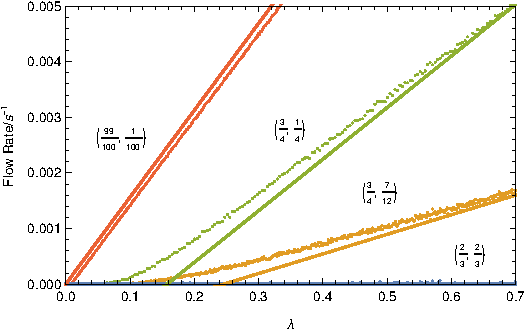
\includegraphics[width=0.5\linewidth]{newFlowMean} & 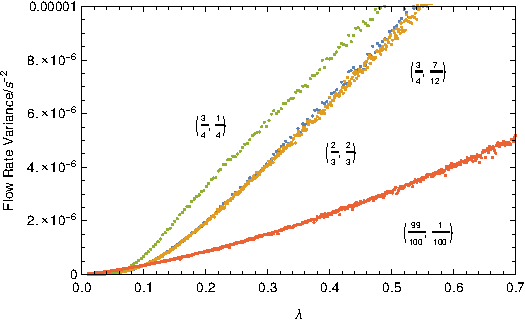
\includegraphics[width=0.5\linewidth]{newFlowVar} \\
    \hline
    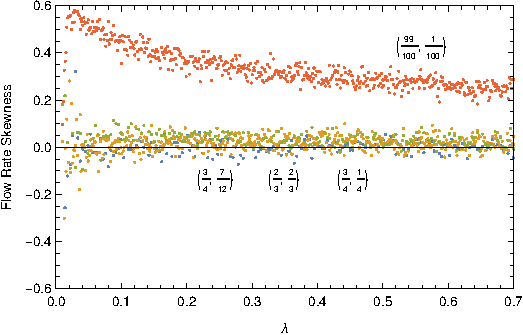
\includegraphics[width=0.5\linewidth]{newFlowSkew} & 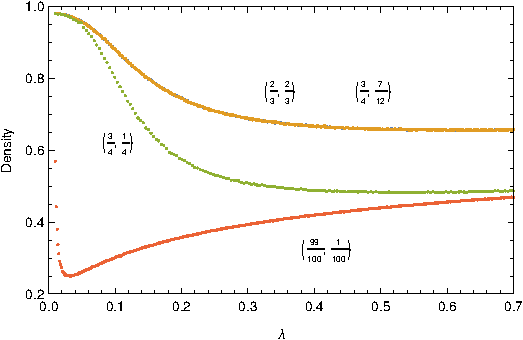
\includegraphics[width=0.5\linewidth]{newDens} \\
    \end{tabular}
\end{center}
    \vspace{-0em}
\end{figure*}

\begin{figure*}[h!]
\vspace{1em}
\caption{\label{fig:fullConstDens} Flow rate variance and average overall densities observed when varying the difference $\delta\rho$ between the boundary concentrations
$(\rho_B, \rho_T) = (\rho_M + \frac{1}{2} \delta\rho, \rho_M - \frac{1}{2} \delta\rho)$ and $\lambda$. $\rho_M=\frac{1}{2}$, as in the paper.}
\begin{center}
 \begin{tabular}{c|c}
    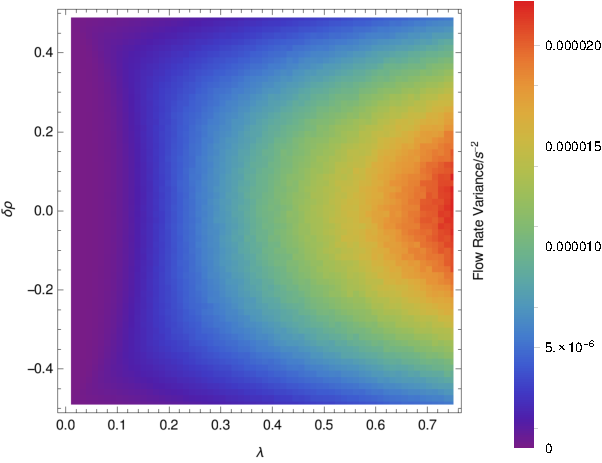
\includegraphics[width=0.5\linewidth]{newConstVar} & 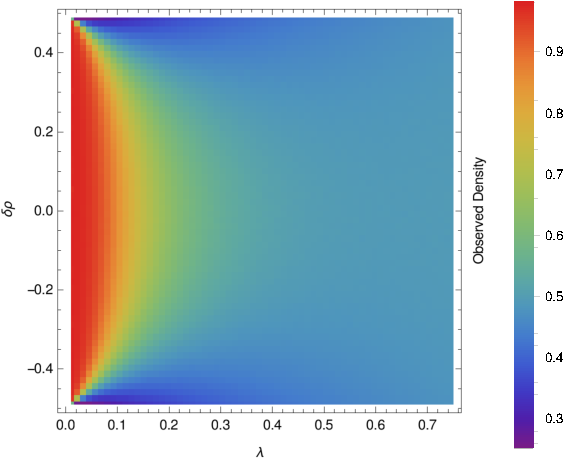
\includegraphics[width=0.5\linewidth]{newConstDens} \\
    \end{tabular}
\end{center}
    \vspace{0em}
\end{figure*}

\begin{figure*}[h!]
\vspace{1em}
\caption{\label{fig:fullDiffCoef}
These images are in addition to our computation of the effective diffusion coefficient $D$. The left shows the overall system density as a function of $\rho_M$ and $\lambda$, whilst the right shows the standard error in our estimate of $D$.
In this setup we ran the KMC simulation for
$1.6\times10^8$ equilibration steps, followed by $10$ sets of alternating measurement and relaxation runs, of lengths $8\times10^7$ and $1.6\times10^7$ steps respectively. These results are consistent with calculations performed on smaller
systems, so finite-size effects should be suppressed.
}

\begin{center}
 \begin{tabular}{c@{\hspace{1em}}c}
    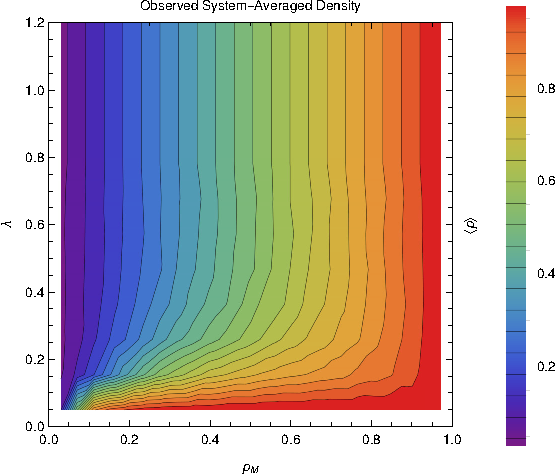
\includegraphics[width=0.5\linewidth]{newFlowDens} & 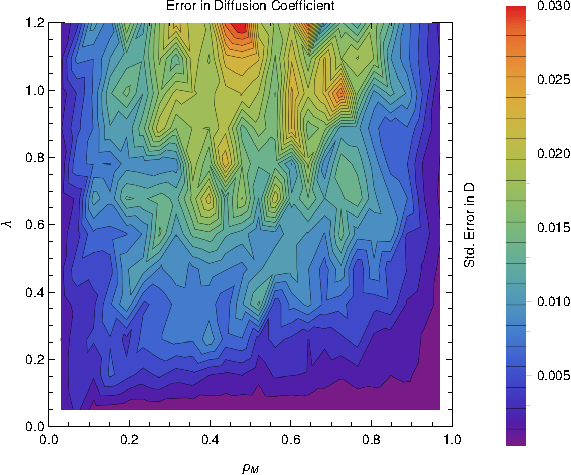
\includegraphics[width=0.5\linewidth]{newFlowErr} 
    \end{tabular}
\end{center}
    \vspace{0em}
\end{figure*}

\textit{More flow plots.} For the interested reader we have included for spacetime flow diagrams, show in Fig.~\ref{fig:flowPatterns}. When $\lambda=0.05$, the medium consists of solid blocks surrounded by empty spaces containing a dilute
gas of particles; at $\lambda=0.35$ it is not so different from normal diffusion.
The most interesting images are those for the intermediate $\lambda$; here we see a ``lumpy'' or ``foamy'' structure, in which small blocks
of particles are being constantly created and destroyed whilst a rather minimal flow occurs across the system.
The simulations did not show any hard phase transition as we vary $\lambda$; rather, it seems that this ``foamy''
behavior is part of a continuous range between the extremes, containing medium-range correlations between particles.
Unfortunately, computing equal-time correlation functions to the accuracy required
to draw conclusions about these correlations has proven to be extremely difficult, so we cannot find a quantitative description of the foam beyond the flow rate and density data we have discussed in this paper.
In all images in Fig.~\ref{fig:flowPatterns}, long straight segments of white of black can be seen.  The represent coherent motion at a characteristic velocity given by their gradient. There is nothing in the MFT to suggest what this velocity
should be, and it is much smaller than the simulated system's length divided by the elapsed time,  $\frac{L}{T}$, thus it must be an emergent property arising from correlated motion of self-assembled regions of  high- or low-density material.
However, it has again proved difficult to analyze this numerically.


\begin{figure*}[h!]
\caption{\label{fig:flowPatterns} The spacetime flow patterns, for $\lambda$-values of $0.05$, $0.15$, $0.25$ and $0.35$ going clockwise from top left.
In each plot time runs along the $x$-axis, space along the $y$-axis, with the bottom boundary being held with a concentration of $\frac{1}{4}$ and the top at $\frac{3}{4}$. White represents full occupation, black empty, and gray shades partial
occupation. The degree of occupation was calculated by taking the \texttt{KMCLib} record of a particular site's occupation (i.e. the Gillespie times at
which the site changed occupation), assigning $0$ and $1$ to particles and vacancies respectively, linearly interpolating this and then integrating over times longer than a single Gillespie step but much shorter than the total time in question.
In each case the total time elapsed is that taken by $2^6$ Gillespie steps, and each short-time-average has been done over the total time divided by $512$, the number of lattice sites; this means that on average a site would change state 8 times
per pixel, although of course the real distribution is not nearly this even.
Time has been rescaled this way in order to allow fair comparison of different $\lambda$-values.}
\begin{center}
 \begin{tabular}{c@{\hspace{0.35em}}c}
    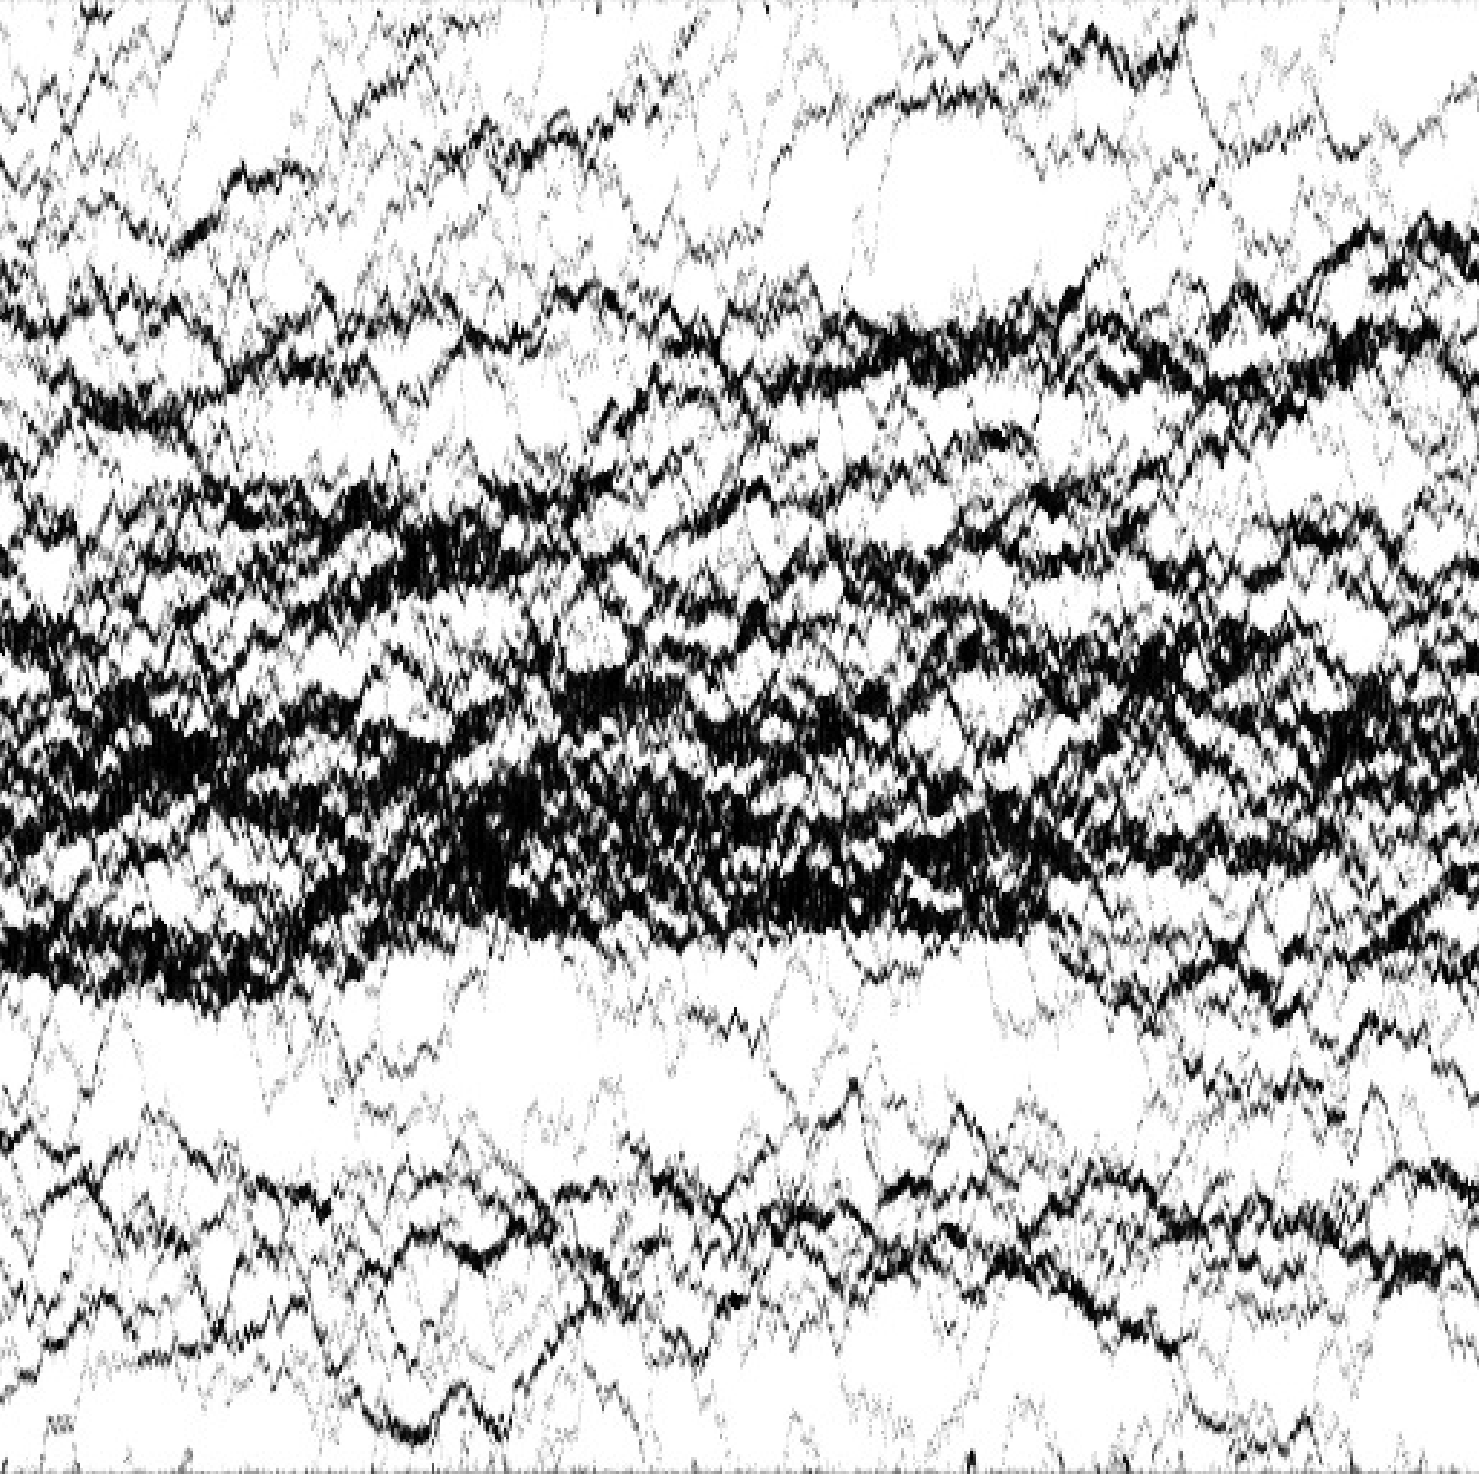
\includegraphics[height=0.3\paperheight]{l05-crop} & 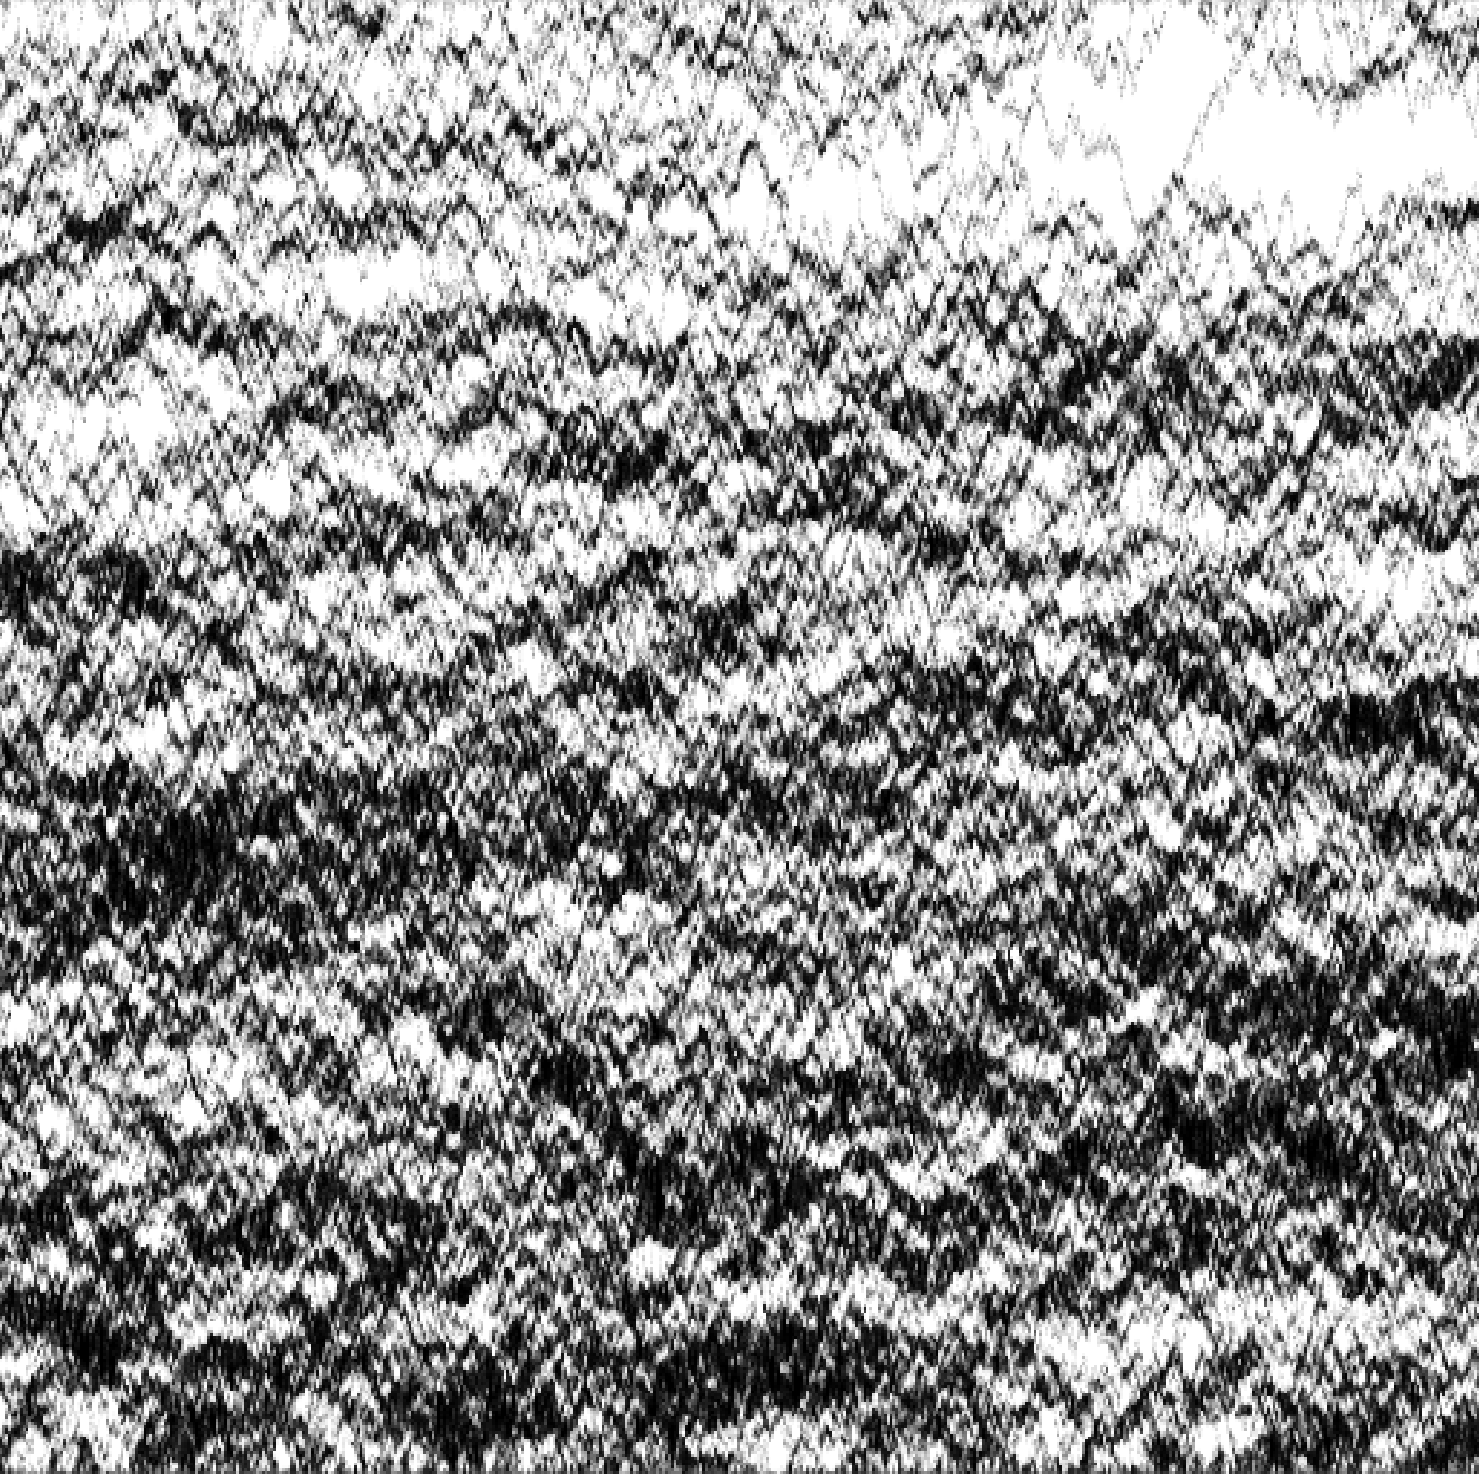
\includegraphics[height=0.3\paperheight]{l15-crop} \\
    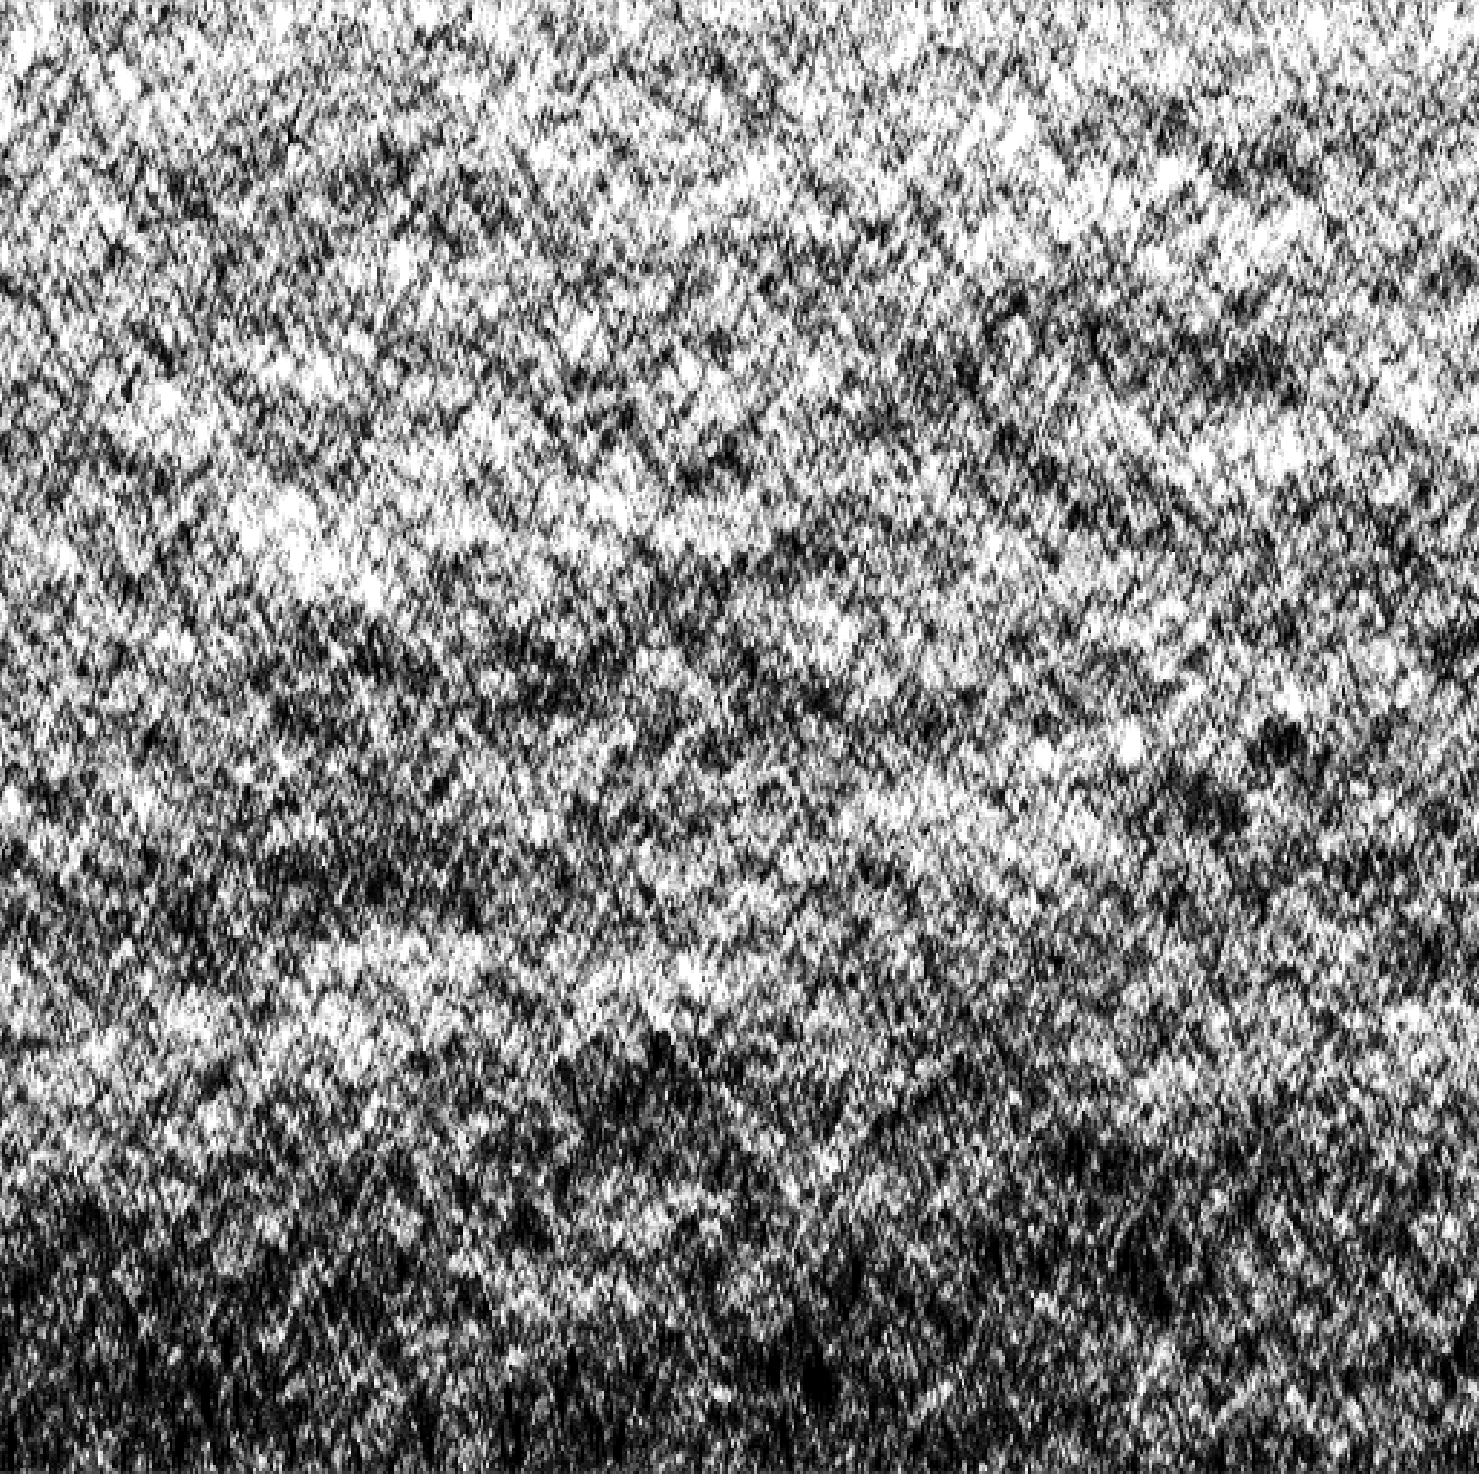
\includegraphics[height=0.3\paperheight]{l35-crop} & 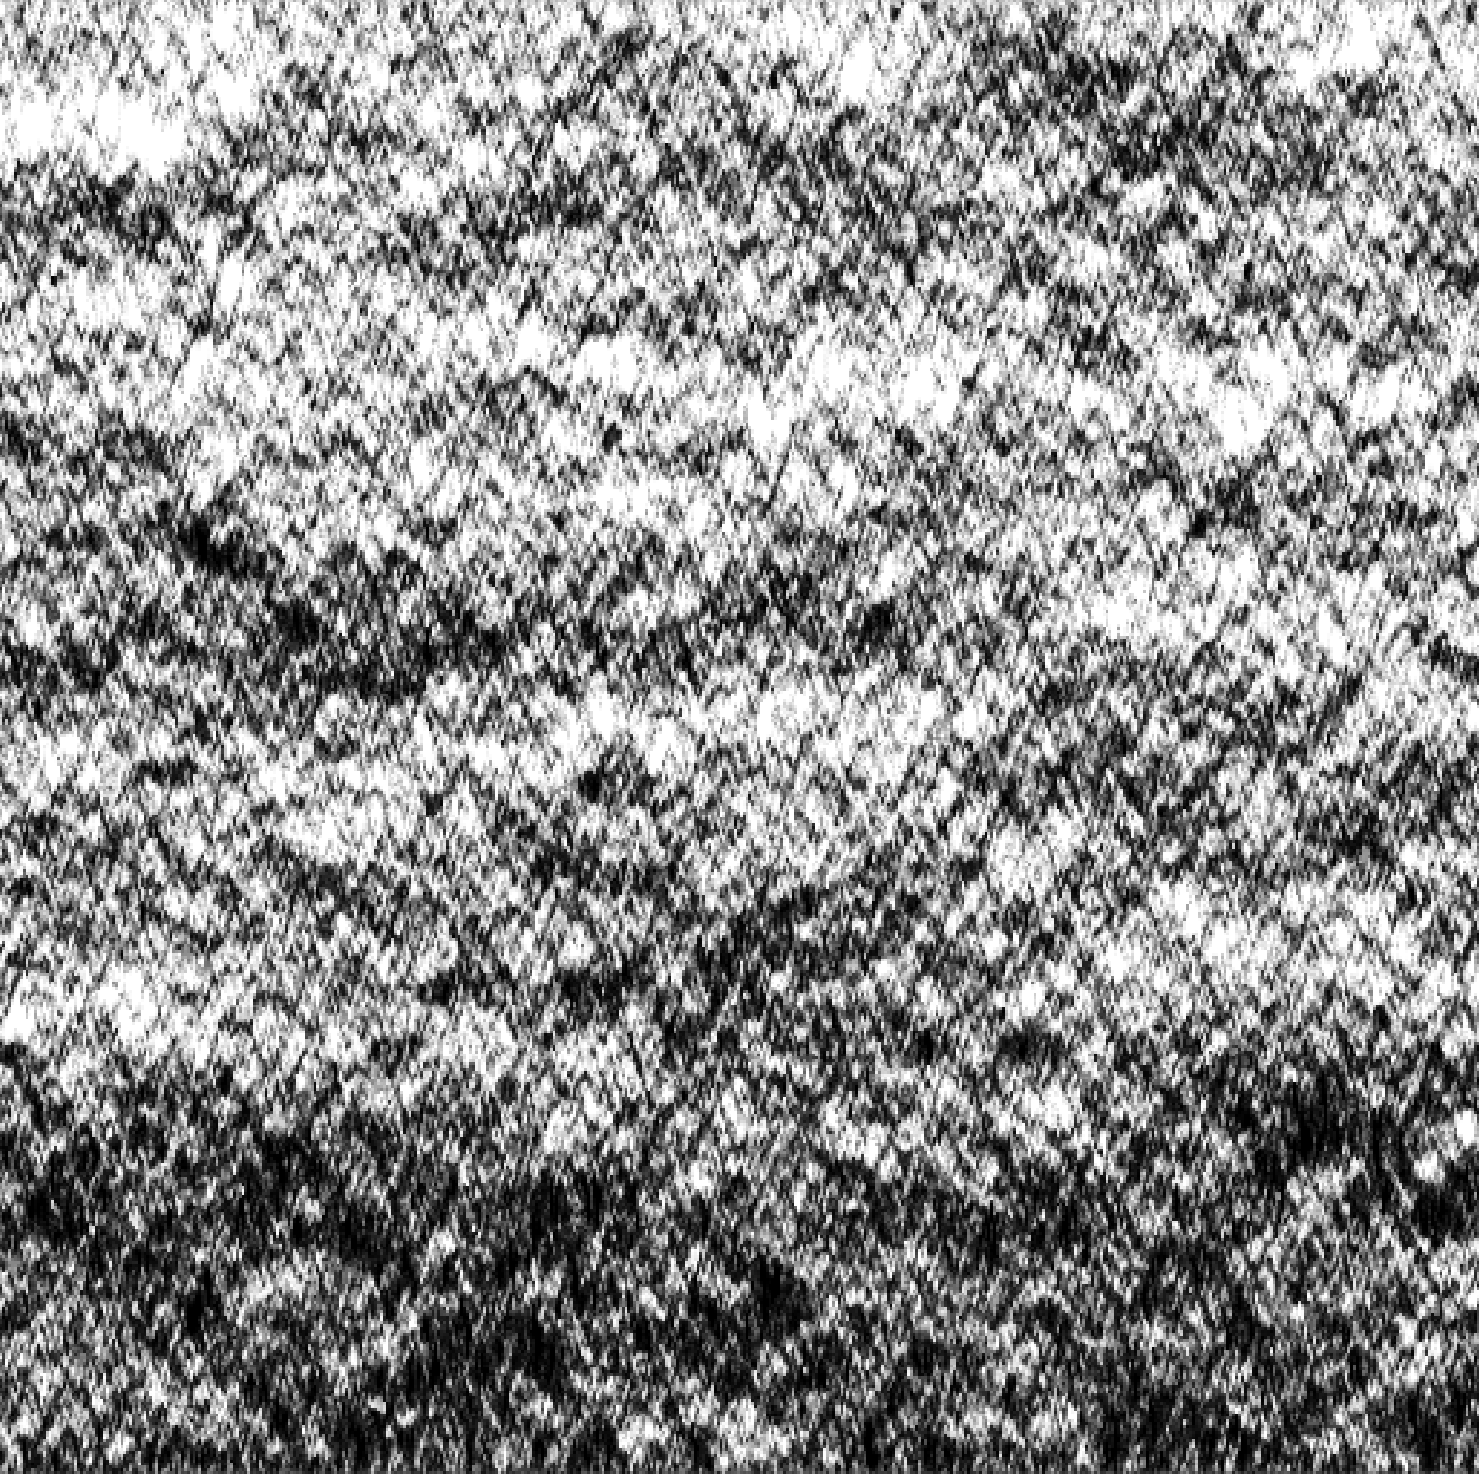
\includegraphics[height=0.3\paperheight]{l25-crop} \\
    \end{tabular}
\end{center}
    \vspace{0em}
\end{figure*}

\textit{Non-Uniqueness of the MFT Density Profile.}
Recall that, according to the MFT,
\begin{equation}
 \int \! \!  \mathrm{d}x \ J(x) = (x-x_0)J_0 = -\frac{a^2}{\tau_0} \rho \left[1+\zeta \rho\left(\rho-2\right)\right], \label{cubic}
\end{equation}
which we would like to solve for $\rho(x)$. We can do this uniquely so long as the right hand side is monotonic for $\rho \in (0, 1)$. Monotonicity requires that the sign of the derivative of the RHS wrt $\rho$ does not change in that region.
This derivative is of course
\begin{equation}
 \frac{\mathrm{d} \mathrm{RHS}}{\mathrm{d} \rho} = -\frac{a^2}{\tau_0} \rho \left[1+\zeta \rho\left(\rho-2\right)\right] = -\frac{a^2}{\tau_0} \left[ 3 \zeta (\rho-\frac{2}{3})^2 + (1-\frac{4}{3} \zeta) \right].
\end{equation}
The term in square brackets is always $1$ at $\rho=0$ and $\lambda$ at $\rho=1$, which are both positive.
If $\zeta<0$, the term is an n-shaped parabola with both boundaries positive; therefore it is always positive, and there is no sign change.
For $\zeta>0$ (the case of interest for us), we can see from completing the square that the term is always positive unless $\zeta > \frac{3}{4}$, in which case there is a sign change and therefore a loss of monotonicity.
Thus for $\zeta > \frac{3}{4}$ (and correspondingly $\lambda<\frac{1}{4}$) the MFT does not have a unique steady state solution given a set of Dirichlet boundary conditions, and so we cannot expect the MFT to predict the density profile
in that regime.

\textit{Particle Density in Bounded Domain at Extreme $\lambda$-Values.}
We scanned across a wide range of $\lambda$ with three sets of boundary conditions: $(\frac{3}{10}, \frac{1}{10})$, $(\frac{3}{4}, \frac{1}{4})$ and $(\frac{9}{10}, \frac{7}{10})$. The resulting mean flow rate is show in
Fig.~\ref{fig:largeFlow}, and mean density in Fig.~\ref{fig:largeDensity}. We once again see the transitions between power law behaviors, as discussed in the main body of the paper. Note that the MFT is never a particularly good
fit for the $(\frac{3}{4}, \frac{1}{4})$ configuration; this may be because the difference between the boundaries is greater than in the other cases. The other MFTs are good fits in the high-$\lambda$ regime until we start reaching $\lambda~\sim~1000$,
at which point they seem to start converging to the same flow regardless of boundary conditions. In each case for low-$\lambda$ we have a power-law regime, each with with an exponent around $4$, and then at extreme low-$\lambda$ we lose
a consistent signal because of noise, which we attribute to lack of system convergence due to critically slow flow.
\begin{figure*}[h!]
\vspace{1em}
\caption{\label{fig:largeFlow} Flow rate as a function of $\lambda$ for systems with boundary conditions $(\frac{3}{10}, \frac{1}{10})$, $(\frac{3}{4}, \frac{1}{4})$ and $(\frac{9}{10}, \frac{7}{10})$, colored in blue, gold and green
respectively.}
    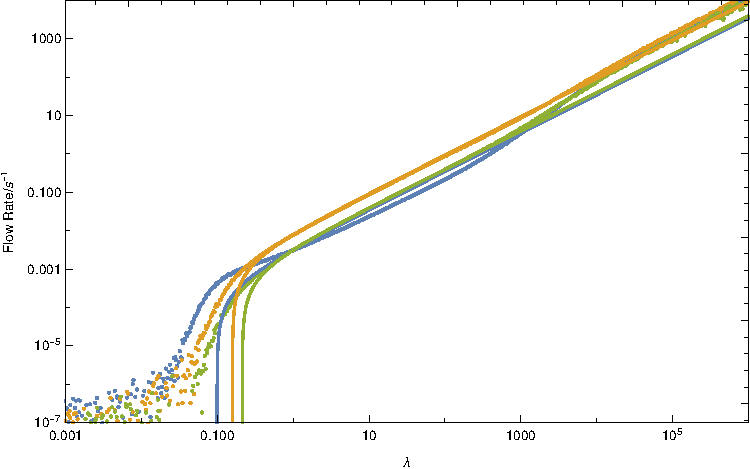
\includegraphics[width=0.95\linewidth]{largeRangeFlow}
    \vspace{0em}
\end{figure*}
\begin{figure*}[h!]
\vspace{1em}
\caption{\label{fig:largeDensity} Density as a function of $\lambda$ for systems with boundary conditions $(\frac{3}{10}, \frac{1}{10})$, $(\frac{3}{4}, \frac{1}{4})$ and $(\frac{9}{10}, \frac{7}{10})$, colored in blue, gold and green
respectively.}
    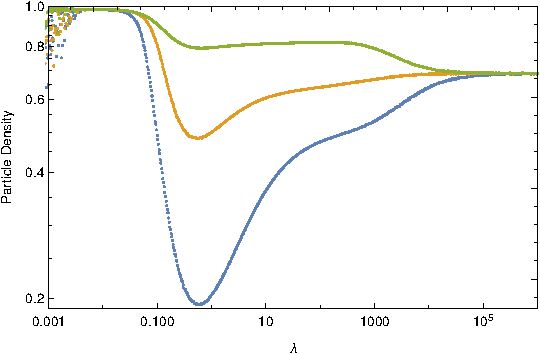
\includegraphics[width=0.95\linewidth]{largeRangeDensity}
    \vspace{0em}
\end{figure*}
So far as the density is concerned, at $\lambda=1$ in each case it is about what we would expect (the average of the two boundary densities). It is minimized around $\lambda = 0.6$, and then as $\lambda$ is reduced each density appears to 
converge to $1$ regardless of boundary conditions (before we encounter the same convergence issue at extreme low-$\lambda$). As we go to high-$\lambda$, on the other hand, we see a similar convergence, but this time towards $\rho \sim 0.7$.
This is interesting, as a density of $\rho=\frac{2}{3}$ is predicted by the MFT to be where maximal flow should occur for $\lambda>1$; thus it would appear that the system self-organizes to facilitate maximal flow, which is something which
is hypothesized to occur in other nonequilibrium statmech systems. This also helps to explain the large deviations from the MFT flow predictions we encounter at high-$\lambda$, as the system in practice has a different density to the one assumed
by the MFT.




\end{document}
%
% ****** End of file apssamp.tex ******
